\documentclass[border=15pt]{standalone}
\usepackage{amsmath, amssymb}
\usepackage{tikz}
\usetikzlibrary{arrows.meta}

\definecolor{block0}{HTML}{E53935}
\definecolor{block1}{HTML}{1E88E5}

\begin{document}
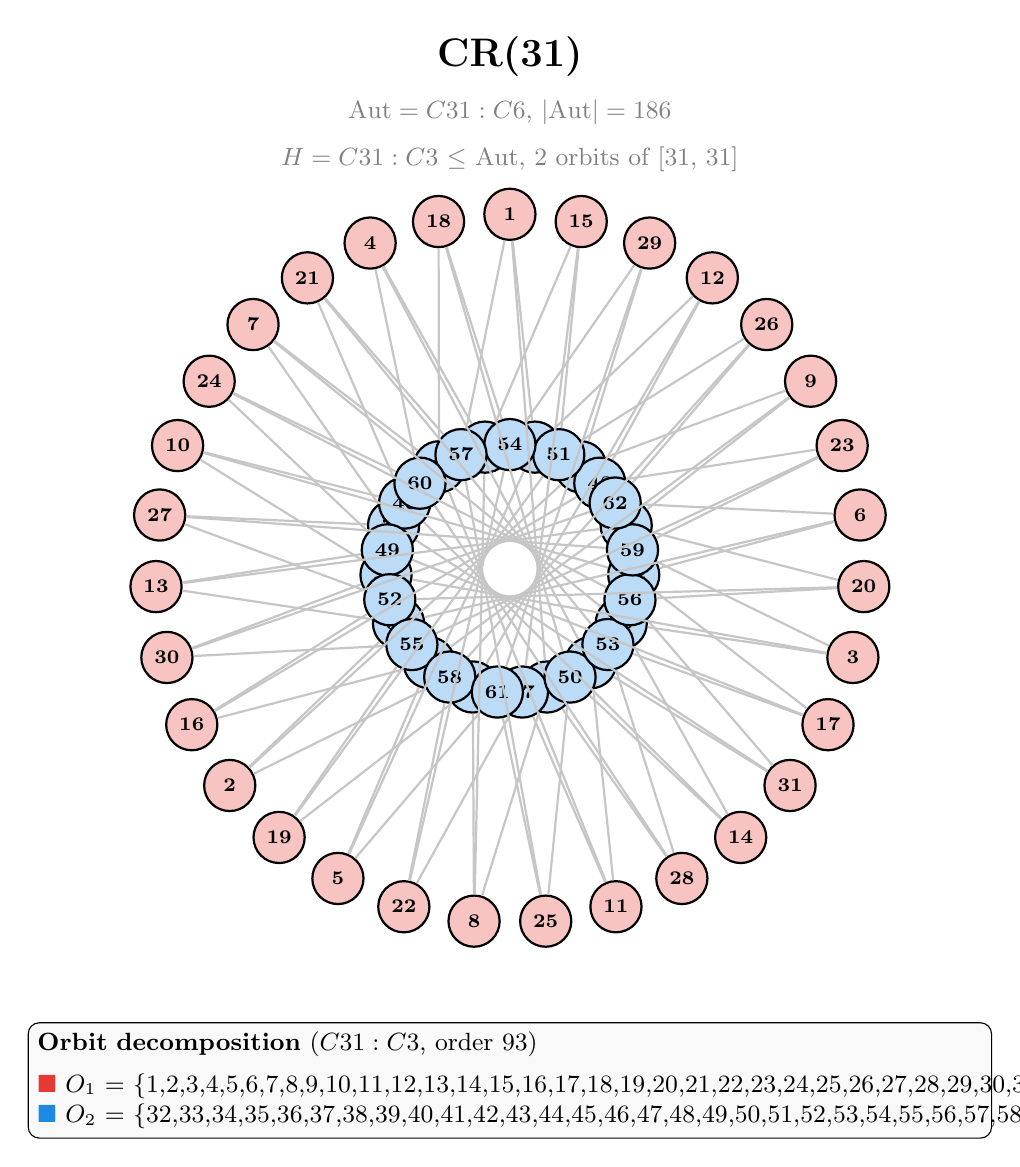
\begin{tikzpicture}[
  vertex/.style={circle, draw, thick, minimum size=6.5mm, inner sep=0pt,
                 font=\scriptsize\bfseries},
  edge/.style={thick, gray!45},
  title/.style={font=\Large\bfseries},
  subtitle/.style={font=\small, text=gray},
]

\node[title] at (0, 6.5) {CR(31)};
\node[subtitle] at (0, 5.8) {$\mathrm{Aut} = C31 : C6$, $|\mathrm{Aut}| = 186$};
\node[subtitle] at (0, 5.2) {$H = C31 : C3$ $\leq$ $\mathrm{Aut}$, 2 orbits of [31, 31]};

\node[vertex, fill=block0!30] (v1) at (0.000, 4.500) {1};
\node[vertex, fill=block0!30] (v2) at (-3.558, -2.754) {2};
\node[vertex, fill=block0!30] (v3) at (4.356, -1.128) {3};
\node[vertex, fill=block0!30] (v4) at (-1.775, 4.135) {4};
\node[vertex, fill=block0!30] (v5) at (-2.184, -3.935) {5};
\node[vertex, fill=block0!30] (v6) at (4.448, 0.681) {6};
\node[vertex, fill=block0!30] (v7) at (-3.262, 3.100) {7};
\node[vertex, fill=block0!30] (v8) at (-0.455, -4.477) {8};
\node[vertex, fill=block0!30] (v9) at (3.819, 2.380) {9};
\node[vertex, fill=block0!30] (v10) at (-4.220, 1.563) {10};
\node[vertex, fill=block0!30] (v11) at (1.347, -4.294) {11};
\node[vertex, fill=block0!30] (v12) at (2.571, 3.693) {12};
\node[vertex, fill=block0!30] (v13) at (-4.494, -0.228) {13};
\node[vertex, fill=block0!30] (v14) at (2.931, -3.414) {14};
\node[vertex, fill=block0!30] (v15) at (0.906, 4.408) {15};
\node[vertex, fill=block0!30] (v16) at (-4.040, -1.982) {16};
\node[vertex, fill=block0!30] (v17) at (4.040, -1.982) {17};
\node[vertex, fill=block0!30] (v18) at (-0.906, 4.408) {18};
\node[vertex, fill=block0!30] (v19) at (-2.931, -3.414) {19};
\node[vertex, fill=block0!30] (v20) at (4.494, -0.228) {20};
\node[vertex, fill=block0!30] (v21) at (-2.571, 3.693) {21};
\node[vertex, fill=block0!30] (v22) at (-1.347, -4.294) {22};
\node[vertex, fill=block0!30] (v23) at (4.220, 1.563) {23};
\node[vertex, fill=block0!30] (v24) at (-3.819, 2.380) {24};
\node[vertex, fill=block0!30] (v25) at (0.455, -4.477) {25};
\node[vertex, fill=block0!30] (v26) at (3.262, 3.100) {26};
\node[vertex, fill=block0!30] (v27) at (-4.448, 0.681) {27};
\node[vertex, fill=block0!30] (v28) at (2.184, -3.935) {28};
\node[vertex, fill=block0!30] (v29) at (1.775, 4.135) {29};
\node[vertex, fill=block0!30] (v30) at (-4.356, -1.128) {30};
\node[vertex, fill=block0!30] (v31) at (3.558, -2.754) {31};
\node[vertex, fill=block1!30] (v32) at (-1.477, 0.547) {32};
\node[vertex, fill=block1!30] (v33) at (0.471, -1.503) {33};
\node[vertex, fill=block1!30] (v34) at (0.900, 1.293) {34};
\node[vertex, fill=block1!30] (v35) at (-1.573, -0.080) {35};
\node[vertex, fill=block1!30] (v36) at (1.026, -1.195) {36};
\node[vertex, fill=block1!30] (v37) at (0.317, 1.543) {37};
\node[vertex, fill=block1!30] (v38) at (-1.414, -0.694) {38};
\node[vertex, fill=block1!30] (v39) at (1.414, -0.694) {39};
\node[vertex, fill=block1!30] (v40) at (-0.317, 1.543) {40};
\node[vertex, fill=block1!30] (v41) at (-1.026, -1.195) {41};
\node[vertex, fill=block1!30] (v42) at (1.573, -0.080) {42};
\node[vertex, fill=block1!30] (v43) at (-0.900, 1.293) {43};
\node[vertex, fill=block1!30] (v44) at (-0.471, -1.503) {44};
\node[vertex, fill=block1!30] (v45) at (1.477, 0.547) {45};
\node[vertex, fill=block1!30] (v46) at (-1.337, 0.833) {46};
\node[vertex, fill=block1!30] (v47) at (0.159, -1.567) {47};
\node[vertex, fill=block1!30] (v48) at (1.142, 1.085) {48};
\node[vertex, fill=block1!30] (v49) at (-1.557, 0.238) {49};
\node[vertex, fill=block1!30] (v50) at (0.764, -1.377) {50};
\node[vertex, fill=block1!30] (v51) at (0.621, 1.447) {51};
\node[vertex, fill=block1!30] (v52) at (-1.525, -0.395) {52};
\node[vertex, fill=block1!30] (v53) at (1.245, -0.964) {53};
\node[vertex, fill=block1!30] (v54) at (0.000, 1.575) {54};
\node[vertex, fill=block1!30] (v55) at (-1.245, -0.964) {55};
\node[vertex, fill=block1!30] (v56) at (1.525, -0.395) {56};
\node[vertex, fill=block1!30] (v57) at (-0.621, 1.447) {57};
\node[vertex, fill=block1!30] (v58) at (-0.764, -1.377) {58};
\node[vertex, fill=block1!30] (v59) at (1.557, 0.238) {59};
\node[vertex, fill=block1!30] (v60) at (-1.142, 1.085) {60};
\node[vertex, fill=block1!30] (v61) at (-0.159, -1.567) {61};
\node[vertex, fill=block1!30] (v62) at (1.337, 0.833) {62};

\draw[edge] (v1) -- (v33);
\draw[edge] (v1) -- (v37);
\draw[edge] (v1) -- (v57);
\draw[edge] (v2) -- (v34);
\draw[edge] (v2) -- (v38);
\draw[edge] (v2) -- (v58);
\draw[edge] (v3) -- (v35);
\draw[edge] (v3) -- (v39);
\draw[edge] (v3) -- (v59);
\draw[edge] (v4) -- (v36);
\draw[edge] (v4) -- (v40);
\draw[edge] (v4) -- (v60);
\draw[edge] (v5) -- (v37);
\draw[edge] (v5) -- (v41);
\draw[edge] (v5) -- (v61);
\draw[edge] (v6) -- (v38);
\draw[edge] (v6) -- (v42);
\draw[edge] (v6) -- (v62);
\draw[edge] (v7) -- (v32);
\draw[edge] (v7) -- (v39);
\draw[edge] (v7) -- (v43);
\draw[edge] (v8) -- (v33);
\draw[edge] (v8) -- (v40);
\draw[edge] (v8) -- (v44);
\draw[edge] (v9) -- (v34);
\draw[edge] (v9) -- (v41);
\draw[edge] (v9) -- (v45);
\draw[edge] (v10) -- (v35);
\draw[edge] (v10) -- (v42);
\draw[edge] (v10) -- (v46);
\draw[edge] (v11) -- (v36);
\draw[edge] (v11) -- (v43);
\draw[edge] (v11) -- (v47);
\draw[edge] (v12) -- (v37);
\draw[edge] (v12) -- (v44);
\draw[edge] (v12) -- (v48);
\draw[edge] (v13) -- (v38);
\draw[edge] (v13) -- (v45);
\draw[edge] (v13) -- (v49);
\draw[edge] (v14) -- (v39);
\draw[edge] (v14) -- (v46);
\draw[edge] (v14) -- (v50);
\draw[edge] (v15) -- (v40);
\draw[edge] (v15) -- (v47);
\draw[edge] (v15) -- (v51);
\draw[edge] (v16) -- (v41);
\draw[edge] (v16) -- (v48);
\draw[edge] (v16) -- (v52);
\draw[edge] (v17) -- (v42);
\draw[edge] (v17) -- (v49);
\draw[edge] (v17) -- (v53);
\draw[edge] (v18) -- (v43);
\draw[edge] (v18) -- (v50);
\draw[edge] (v18) -- (v54);
\draw[edge] (v19) -- (v44);
\draw[edge] (v19) -- (v51);
\draw[edge] (v19) -- (v55);
\draw[edge] (v20) -- (v45);
\draw[edge] (v20) -- (v52);
\draw[edge] (v20) -- (v56);
\draw[edge] (v21) -- (v46);
\draw[edge] (v21) -- (v53);
\draw[edge] (v21) -- (v57);
\draw[edge] (v22) -- (v47);
\draw[edge] (v22) -- (v54);
\draw[edge] (v22) -- (v58);
\draw[edge] (v23) -- (v48);
\draw[edge] (v23) -- (v55);
\draw[edge] (v23) -- (v59);
\draw[edge] (v24) -- (v49);
\draw[edge] (v24) -- (v56);
\draw[edge] (v24) -- (v60);
\draw[edge] (v25) -- (v50);
\draw[edge] (v25) -- (v57);
\draw[edge] (v25) -- (v61);
\draw[edge] (v26) -- (v51);
\draw[edge] (v26) -- (v58);
\draw[edge] (v26) -- (v62);
\draw[edge] (v27) -- (v32);
\draw[edge] (v27) -- (v52);
\draw[edge] (v27) -- (v59);
\draw[edge] (v28) -- (v33);
\draw[edge] (v28) -- (v53);
\draw[edge] (v28) -- (v60);
\draw[edge] (v29) -- (v34);
\draw[edge] (v29) -- (v54);
\draw[edge] (v29) -- (v61);
\draw[edge] (v30) -- (v35);
\draw[edge] (v30) -- (v55);
\draw[edge] (v30) -- (v62);
\draw[edge] (v31) -- (v32);
\draw[edge] (v31) -- (v36);
\draw[edge] (v31) -- (v56);

\node[draw, rounded corners, fill=gray!5, text width=12cm, align=left, font=\small]
  at (0, -6.5) {
  \textbf{Orbit decomposition} ($C31 : C3$, order 93) \\[4pt]
  \textcolor{block0}{$\blacksquare$} $O_{1}$ = \{1,2,3,4,5,6,7,8,9,10,11,12,13,14,15,16,17,18,19,20,21,22,23,24,25,26,27,28,29,30,31\} \\
  \textcolor{block1}{$\blacksquare$} $O_{2}$ = \{32,33,34,35,36,37,38,39,40,41,42,43,44,45,46,47,48,49,50,51,52,53,54,55,56,57,58,59,60,61,62\}
};

\end{tikzpicture}
\end{document}